\documentclass[10pt,a4paper]{article}
\usepackage[utf8]{inputenc}
\usepackage[italian]{babel}
\usepackage{amsmath}
\usepackage{amsfonts}
\usepackage{amssymb}
\usepackage{graphicx}
\usepackage[left=2cm,right=2cm,top=2cm,bottom=2cm]{geometry}
\newcommand{\rem}[1]{[\emph{#1}]}

\author{Gruppo AC \\ Belliardo Federico, Franchi Giulia, Mazzoncini Francesco}
\title{Esercitazione N.5: Transistor JFET.}
\begin{document}

\maketitle

\section{Scopo e strumentazione}
Studiare le caratteristiche e realizzare un amplificatore con il JFET a canale N 2N3819.

\section{Studio funzionamento del JFET}
\paragraph{Montaggio e ossevazioni qualitative.}
E' stato montato il circuito in fig. \ref{circuito1}, con  $R_1 = 0.994\pm0.008 \, k\Omega$, $V_1 = 15.11\pm0.08 \, V$ e $V_2 = -15.01 \pm 0.08 \, V$ \footnote{Misure eseguite con il multimetro digitale}. Le due sorgenti di tensione DC sono state ottenute dalle due boccole del generatore in dotazione. Le resistenze massime e minime del potenziometro (indicato con $R_2$) sono:  $R_{max} = 1.95 \pm 0.01 \, k\Omega$ e $R_{min} = 0.3 \pm 0.3 \, \Omega$

\begin{figure}[h]
\centering
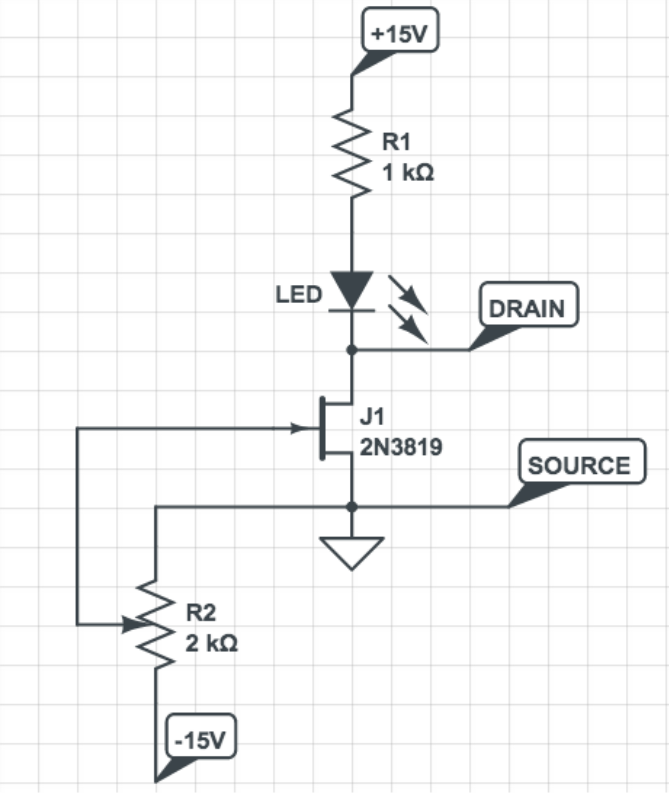
\includegraphics[scale=0.3]{circuito1.png}
\caption{Schema di amplificatore con JFET in corrente continua.\label{circuito1}}
\end{figure}

Variando la resistenza del potenziometro (partitore di tensione) cambia la tensione di \emph{gate} ($V_{GS}$), dunque il JFET entra in conduzione solamente quando si supera la tensione $V_{GS} > V_{P}$ (tensione di \emph{pinch-off}), quando ciò succede si accende il led. Qualitativamente stimiamo: $V_P \sim 3\,V$. 

\paragraph{Misura della corrente $I_D$ in funzione di $V_{GS}$.}
Si sono prese misure della tensione $V_{GS}$ e di $V_{R1}$ (caduta di potenziale ai capi di $R_1$) utilizzando il multimetro digitale \footnote{Abbiamo evitato l'uso dell'oscilloscopio perchè le nostre misure non fossero affette dall'errore sistematico del $3\%$}, da $V_{R1}$ si è ricavata $I_D = \frac{V_{R1}}{R_1}$. Nella tabella \ref{correnteId} e in fig. \ref{tuttiIdati} sono riporati i dati presi. Gli errori delle misure di tensione nei grafici e nella tabella sono calcolati come specificato nel manuale del multimetro.\\
La retta di carico è: $V_1 - R_1 I_D-V_{\gamma}-V_{DS} = 0$, dove $V_{\gamma} \sim 1.8 \, V$ è la caduta di tensione sul led rosso (caratteristica del led). Questa retta di carico è valida quando il led è acceso cioè quando vi è una corrente $I_D$: sono in zona ohmica o di saturazione, mentre $V_{DS} = V_1$ è la retta di carico quando sono in zona di interdizione.\\

\begin{table}[!htb]\centering
\begin{tabular}{|c|c|c|c|c|c|}
\hline
$ V_{R1} (V)$ & $ \sigma V_{R1} (V) $ & $V_{GS} (V) $ & $\sigma V_{GS} (V)$ & $I_D (mA)$ & $\sigma I_D (mA)$\\ 
\hline
0.013 & 0.001 & -3.27 & 0.02 & 0.013 & 0.001\\
0.078 & 0.001 & -3.13 & 0.02 & 0.079 & 0.001\\
0.264 & 0.002 & -2.94 & 0.02 & 0.266 & 0.003\\
0.462 & 0.003 & -2.81 & 0.02 & 0.465 & 0.005\\
1.02 & 0.01 & -2.51 & 0.02 & 1.03 & 0.01\\
1.69 & 0.01 & -2.23 & 0.01 & 1.70 & 0.02\\
2.94 & 0.02 & -1.81 & 0.01 & 2.96 & 0.03\\
4.34 & 0.02 & -1.37 & 0.01 & 4.37 & 0.04\\
6.22 & 0.03 & -0.872 & 0.004 & 6.26 & 0.06\\
8.01 & 0.04 & -0.413 & 0.002 & 8.06 & 0.08\\
9.36 & 0.05 & -0.037 & 0.001 & 9.42 & 0.09\\
\hline
\end{tabular}
\caption{Dati di corrente $I_D$ e di tensione $V_{GS}$, $V_{R1}$}
\label{correnteId}
\end{table}

\begin{figure}[h]
\centering
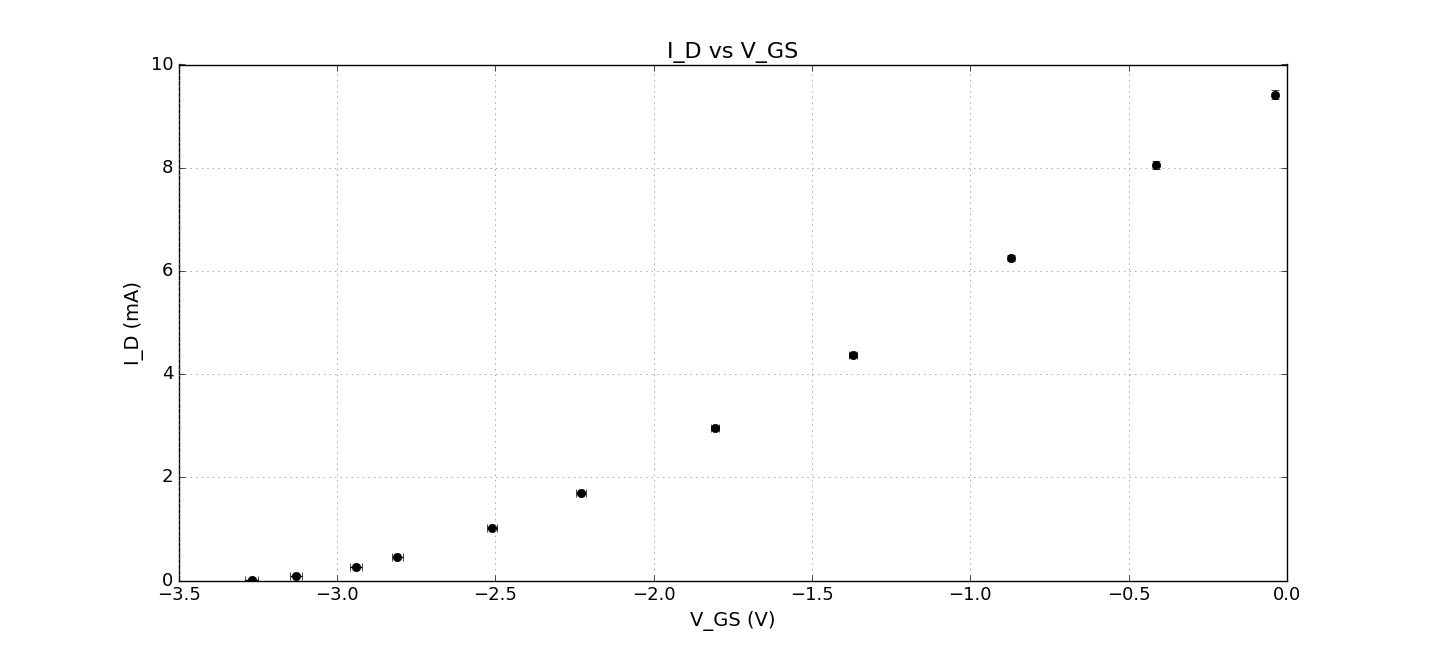
\includegraphics[scale=0.5]{parabolaTutti.png}
\caption{Corrente di drain misurata in funzione della tensione $V_{GS}$.\label{tuttiIdati}}
\end{figure}

\begin{figure}[h]
\centering
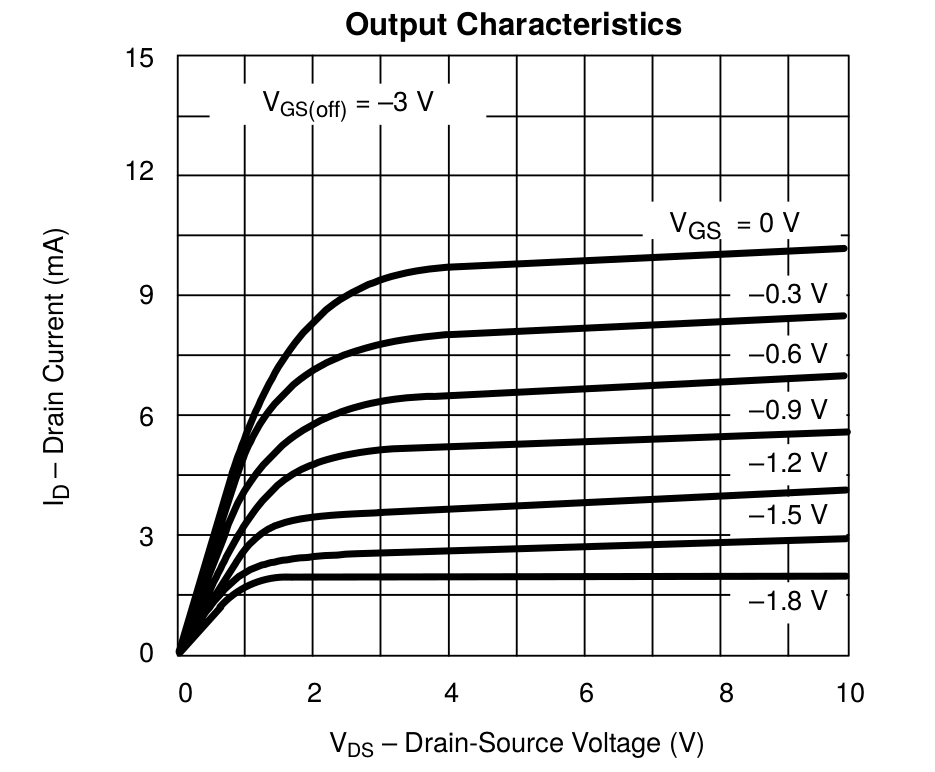
\includegraphics[scale=0.4]{char2.png}
\caption{Curve caratteristiche del JFET dal datasheet.\label{curveCaratteristiche}}
\end{figure}

La fig. \ref{curveCaratteristiche} riporta un'immagine delle curve caratteristiche del JFET nel caso in cui la tensione di \emph{pinch-off} sia $V_P = -3.0\,V$, sul quale è riportata la retta di carico. Si può estrapolare dal grafico che per i valori delle tensioni $V_{GS}$ esplorati (riportati nella tabella \ref{correnteId}) siamo sempre in zona di saturazione e non in zona ohmica, dunque valgono le approssimazioni note dalla teoria del JFET per questo regime (per esempio la dipendenza quadratica di $I_D$ da $V_{GS}$).\\

\begin{figure}[h!]
\centering
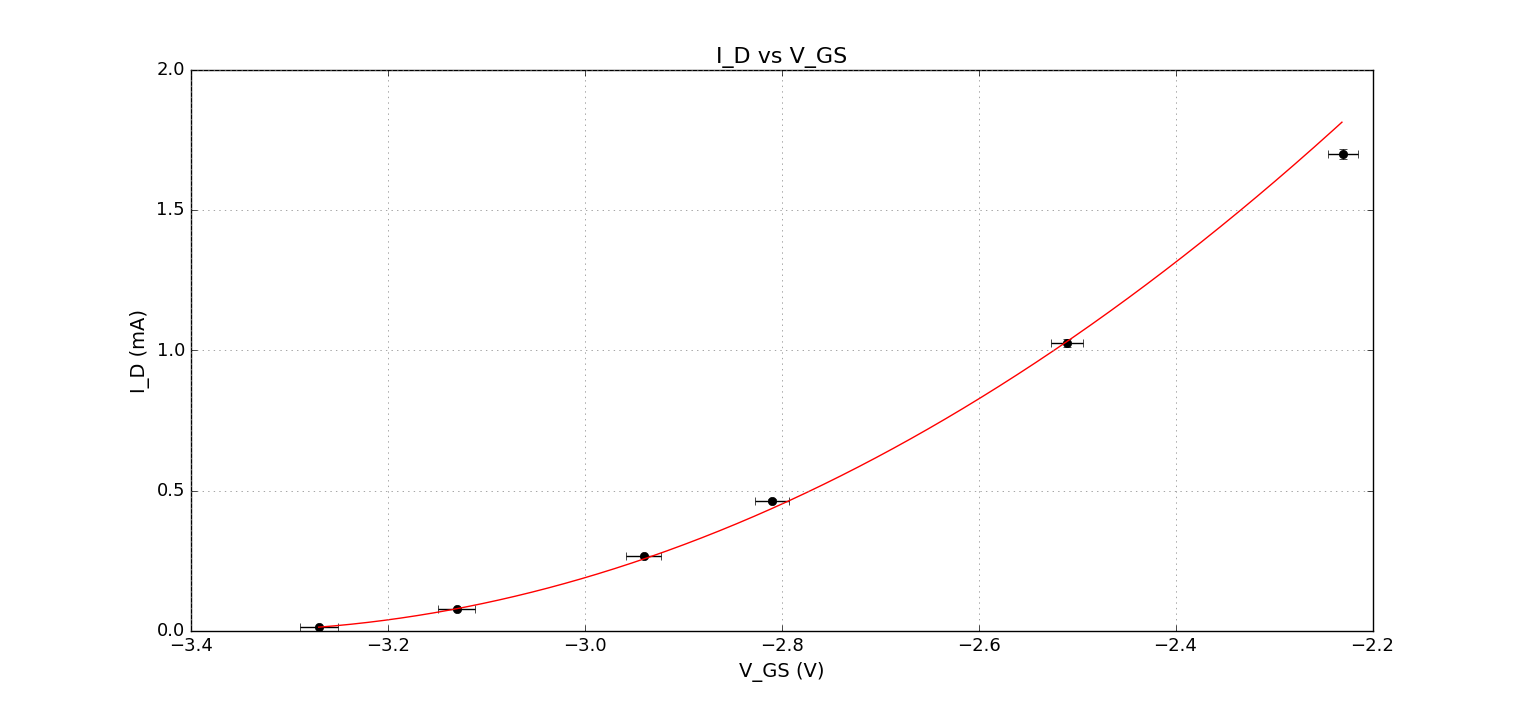
\includegraphics[scale=0.5]{parabolaFit.png}
\caption{Fit parabolico intorno alla tensione di pinch off.\label{correnteIdVgs}}
\end{figure}

E' stato eseguito un fit di una funzione parabolica ($I_D = K_P (V_{GS} - V_P)^2$), considerando solamente i dati attorno alla tensione di \emph{pinch-off}, cioè in una regione in cui ci aspettiamo valga il comportamento ideale. \\
Per il fit numerico si è utilizzata la funzione \emph{curvefit} della libreria \emph{pylab} con l'opzione \emph{$absolute\,sigma = "true"$}, poichè abbiamo considerando gli errori come statistici. Riportiamo il grafico in figura \ref{correnteIdVgs} e di seguito parametri fittati con la relativa matrice di covarianza: $K_P = 1.30 \pm 0.05 \, \frac{mA}{V^2}$, $V_P = -3.39 \pm 0.02 \, V$,  $ \Sigma_{ij} = \left( \begin{array}{cc}
3.46 \cdot 10^{-3} & 8.40 \cdot 10^{-4} \\ 
8.40 \cdot 10^{-4} & 2.69 \cdot 10^{-4}\\
\end{array} \right)$. Con un $\chi^2/ndof = 3/4$.


Il punto del grafico per cui $V_{GS} \sim 0\,V$ corrisponde alla corrente $I_{DSS} = 9.5 \pm 0.2\, mA$ \footnote{L'errore su $I_{DSS}$ è la semidispersione dell'intervallo massimo in cui è ragionevole si trovi $V_{GS} \sim 0\,V$.}, mentre $V_P \sim -3.3\,V$ (tensione a $I_D \sim 0 \, mA$), entrambe stimate dal grafico.\\
Alternativamente si possono utilizzare le informazioni del fit: $I_{DSS} = K_P V_{P}^2 = 15.0 \pm 0.3 \, mA$. I due valori non sono compatibili, perchè il fit esguito non può essere estrapolato fino a tensioni prossime allo zero.\\



Il valore di $V_P$ è molto variabile per costruzione, ma il valore misurato è compatibile con quello tipico indicato nel \emph{datasheet}: $V_{P, datasheet} = -3 \, V$. Per $I_{DSS}$ sono riportati possibili valori tra $2 \, mA$ e $20 \, mA$, entrambi i valori ottenuti sono compatibili.\\

\section{Montaggio amplificatore}

\paragraph{Stima della tensione $V_P$ e della corrente $I_{DSS}$.}
Si è montato il circuito in fig. \ref{circuito2}, con i componenti: $R_1 = 0.994\pm0.008 \, k\Omega $, $R_2 = 1.95\pm0.02 \, k \Omega $, $R_3 = 4.66 \pm 0.04 \, M \Omega$ e $C_1 = 99\pm4 \, nF$ e $V_1 = 15.01\pm0.08 \, V$. \\

Si è regolato il potenziometro in modo che la corrente di quiescenza fosse la metà di $I_{DSS}$, il valore misurato di $V_{R1} = 4.49 \pm 0.03 \, V$, dal quale si ottiene: $I_D = 4.52\pm0.04\,mA$. La resistenza a cui si osserva ciò è: $R_{part} = 237\pm2 \Omega$ (è lasciata costante e sarà usata successivamente). Si è misurata la tensione $V_{GS} = 0.972 \pm 0.005 \,V$. Dalla formula \footnote{In questa formula e nelle seguenti il valore di $I_{DSS}$ è quello stimato dal grafico, mentre $V_P$ è quello ottenuto dal fit.} $V_{GS} = V_{P} \left( 1 - \sqrt{\frac{I_D}{I_{DSS}}} \right)$ (valida in zona di saturazione), ricaviamo il valore atteso per $V_{GS}$ cioè: $V_{GS} = -1.05\pm0.01 \, V$. Le due isure (diretta e indiretta) di $V_{GS}$ sono simili ma non compatibili entro l'errore riportato, probabilemnte è stato sottostumato l'errore su $R_{part}$. \\
Da questi dati si può anche dare una stima della tranconduttanza: $g_m = \frac{i_D}{v_{GS}} = \frac{2I_{DSS}}{\vert V_P \vert} \sqrt{\frac{I_D}{I_{DSS}}} = 3.87\pm0.05\,mS$. Il valore è compatibile con quello indicato dal \emph{datasheet} per la tensione di lavoro scelta.

\begin{figure}
\centering
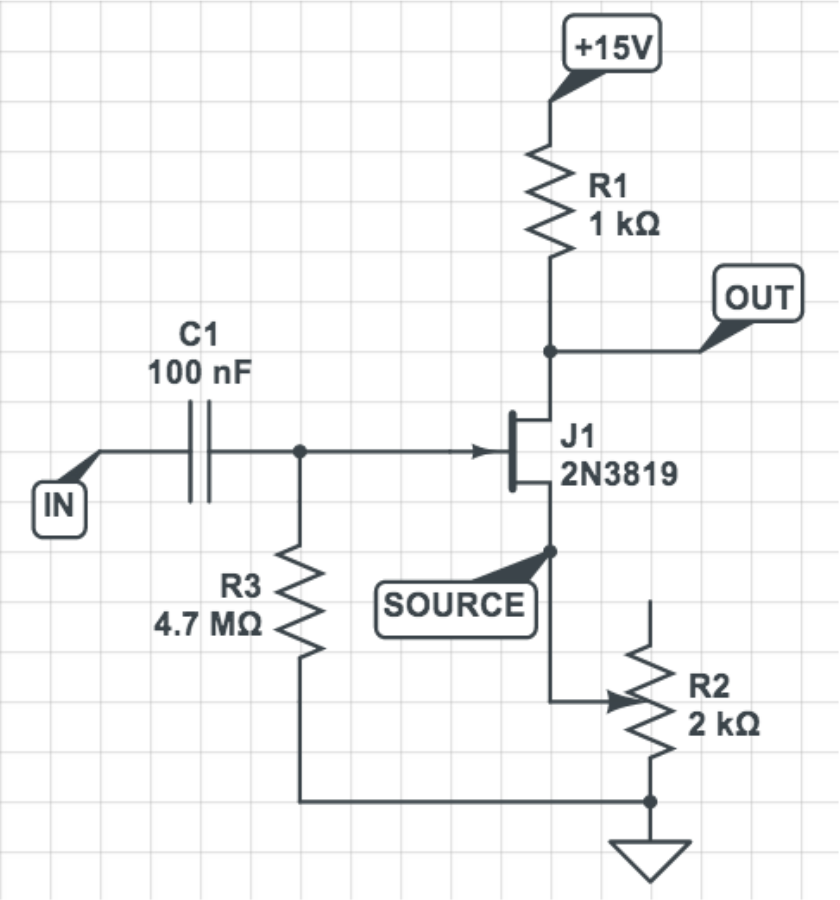
\includegraphics[scale=0.3]{circuito2.png}
\caption{Schema di JFET in corrente continua.\label{circuito2}}
\end{figure}

\section{Misure a frequenza fissa}
Tutte le misure di questa sezione sono prese usando una frequenza fissa di $f_0 = 1.00\pm0.01\, kHz$. L'ingresso del circuito in entrambi i casi è al gate.
\paragraph{Circuito \emph{common source}.}
Si sono prese le misure si tensione in uscita dal \emph{drain}. I dati sono riportati nella tabella \ref{tabellaCommonSource}.

\begin{table}[!htb]\centering
\begin{tabular}{|c|c|c|c|c|c|}
\hline
$V_{IN} (V)$ & $\sigma V_{IN} (V)$ & $V_{OUT} (V)$ & $\sigma V_{OUT} (V)$ & $A_V$ & $\sigma A_V$\\
\hline
0.109 & 0.001 & 0.208 & 0.001 & -1.91 & 0.02\\
0.220 & 0.002 & 0.424 & 0.001 & -1.93 & 0.02\\
0.428 & 0.002 & 0.816 & 0.001 & -1.907 & 0.009\\
0.768 & 0.004 & 1.510 & 0.002 & -1.97 & 0.01\\
0.936 & 0.002 & 1.840 & 0.002 & -1.966 & 0.005\\
1.300 & 0.004 & 2.540 & 0.002 & -1.954 & 0.006\\
\hline
\end{tabular}
\caption{Guadagno JFET in \emph{common source}.}
\label{tabellaCommonSource}
\end{table}

Trascurando la corrente che scorre nel \emph{gate} abbiamo le due equazioni per piccoli segnali: $i_D = g_m v_{gs} = \frac{v_S}{R_{part}}$ e $i_D = g_m v_{gs} = -\frac{v_D}{R_1}$, da queste si ottiene: $A_V = -\frac{v_D}{v_G} = - \frac{R_1 g_m}{1+R_{part} g_m} = -2.01\pm0.02$. \\
Come si vede dalla tabella per gli intervalli di tensione per cui si sono prese le misure l'amplificazione rimane circa costante e il suo valore medio è: $A_V = -1.938\pm0.005$ \footnote{Nella propagazione degli errori si è trascurato l'errore sistematico di calibrazione del  $3\%$ dell'oscilloscopio perchè questo tende a semplificarsi del raporto di due tensioni, questo vale anche per la misura con il \emph{source follower}.}. \\
Si è iniziato ad avere clipping superiore per $V_{clipping, sup} = 5.92\pm0.04 \, V$. Abbiamo impostato l'oscilloscopio in DC e si è osservato che il \emph{clipping} taglia il segnale a $15\,V$ \footnote{La misura della tensione di $V_{OUT}$ al \emph{clipping} è stata eseguita con l'oscilloscoio in DC, poichè essendo il segnale non simmetrico l'eliminazione dell'offset avrebbe falsato la misura e l'interpretazione del \emph{clipping}.} che è la massima tensione erogabile (tensione di alimentazione).\\
Si osserva inversione del segnale, come si vede dalla formula del guadagno in cui compare un segno meno. Questo spiega la presenza del \emph{clipping} superiore infatti per segnali in uscita positivi il segnale di ingresso è negativo duqnue il JFET va in interdizione, non passa più corrente in $R_1$ e la tensione di \emph{drain} è uguale alla tensione $V_1$. 
\paragraph{Circuito \emph{source follower}.}
Nella tabella \ref{tabellaSourceFollower} sono riportati i dati prendendo come uscita il source, si sono ripetute le stesse misure e analisi.

\begin{table}[!htb]\centering
\begin{tabular}{|c|c|c|c|c|c|}
\hline
$V_{IN} (V)$ & $\sigma V_{IN} (V)$ & $V_{OUT} (V)$ & $\sigma V_{OUT} (V)$ & $A_V$ & $\sigma A_V$\\
\hline
0.114 & 0.001 & 0.056 & 0.001 & 0.49 & 0.01\\
0.174 & 0.002 & 0.084 & 0.001 & 0.483 & 0.008\\
0.254 & 0.002 & 0.126 & 0.001 & 0.496 & 0.006\\
0.346 & 0.002 & 0.172 & 0.002 & 0.497 & 0.006\\
0.444 & 0.004 & 0.220 & 0.002 & 0.495 & 0.006\\
0.552 & 0.004 & 0.274 & 0.002 & 0.496 & 0.005\\
\hline
\end{tabular}
\caption{Guadagno JFET in \emph{source follower}.}
\label{tabellaSourceFollower}
\end{table}

Dalle stesse equazioni della sezione precedente otteniamo la relazione: $A_V = \frac{R_{part} g_m}{1+R_{part} g_m}$, dalla quale si può stimare teoricamente il guadagno atteso come: $A_V = 0.478\pm0.004$. \\
La media delle misure è $A_V = 0.493\pm0.003$. In questo caso non si ha inversione, come si può vedere dal segno positivo del guadagno atteso.\\
I due valori di ampiezza non sono in accordo entro l'errore sperimentale, poichè nella propagazione sono stati trascurati gli errori sistematici dell'oscilloscopio al $3\%$, questo vale anche per la sezione \emph{common source}.\\
Si osserva clipping inferiore alla tensione: $V_{clipping, inf} = 6.24\pm0.04\,V $. Il segnale in uscita in questo caso è saturato a $\sim -15\,V$, che è la tensione dell'alimentazione inferiore.\\
Essendo il sagnale non invertito, l'interpretazione del \emph{clipping} è uguale a quella della sezione precendente: per segnali bassi la tensione $V_{GS}$ scende sotto quella di \emph{pinch-off} e il JFET va in interdizone, duqnue non scorre corrente nel potenziometro e la tensione di \emph{source} è uguale a $V_2$.\\
Nella formula per determinare il guadagno vediamo $g_m$ sia a numeratore che a denominatore, dunque non possiamo propagare l'errore considerandoli come indipendenti (sovrastimeremmo troppo l'errore sull'amplificazione). La propagazione statistica eseguita con le derivate parziali (di $A_V(g_m, R_1, R_{part})$) sommate in quadratura li considera come errori non indipendenti, quindi si è eseguito il calcolo in questo modo.\\

\section{Misura impedenza di ingresso}
Trascurando le impedenze tra i terminali del JFET possiamo stimare $R_{int} = \frac{1}{j \omega C} + R_3 \sim R_3 = 4.66\pm0.04 M\Omega$ \footnote{A $f = 1\,kHz$ l'impedenza del condensatore vale $Z_C = 5\,k\Omega$ dunque è trasurabile per entrambe le frequenze.}. Si sono misurate le tensioni in uscita con ($V_1$) e senza ($V_2$) resistenza $R_{S} = 5.20 \pm 0.05 \, M\Omega$ posta in serie al generatore di funzioni. La resistenza in ingresso misurata si ottiene dalla formula del partitore di tensione: $\frac{R_S}{R_IN} = \frac {V_1}{V_2} - 1$ (dove $V_1$ è la tensione misurata senza resistenza $R_S$). Si sono eseguite le misure per le frequenze $f_1 = 1 kHz$ e $f_2 = 10 kHz$.

In tabella \ref{tabellaInterna} sono anche riportate le resistenze attese calcolate teoricamente alle due frequenze:\\

\begin{table}[!htb]\centering
\begin{tabular}{|c|c|c|c|c|}
\hline 
• & $V_1 (V)$ & $V_2 (V)$ & $R_{IN, mis} (M\Omega)$ & $R_{IN, att} (M\Omega)$ \\ 
\hline
$1 kHz$ & $1.43 \pm 0.01$ & $0.648 \pm 0.004$ & $4.31 \pm 0.08$ & $4.66\pm0.04$\\ 
\hline 
$10 kHz$ & $1.43 \pm 0.01$ & $0.206 \pm 0.002$ & $0.87\pm0.02$ & $4.66\pm0.04$ \\ 
\hline 
\end{tabular}\\
\caption{Dati tensioni in uscita e resistenze interne attese e misurate.}
\label{tabellaInterna}
\end{table}

L'impedenza misurata sperimentalmente è minore di quella calcolata teoricamente a causa delle impendenze delle capacità tra i terminali del JFET, che sono poste in parallelo alla resistenzea $R_3$ come si vede in fig. \ref{piccoliSegnali}.

\begin{figure}
\centering
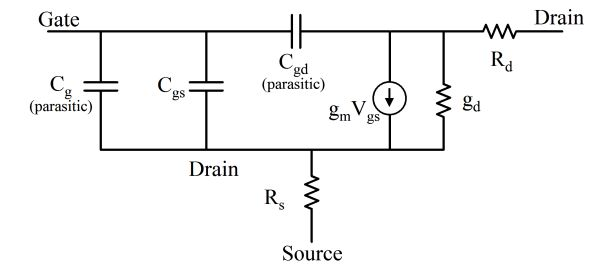
\includegraphics[scale=0.8]{image21.jpg}
\caption{Modello a piccoli segnali del transistor JFET (con capacità parassite).}\label{piccoliSegnali}
\end{figure}

Le capacità parassite sono in parallelo alla resistenza $R_S$, esse sono molto variabili (come riportato nel \emph{datasheet}) ma sono dell'ordine del $pF$, pertanto le tipica impendenza associate sono $Z_C = 100 \, M\Omega$ (a $f=1\, kHz$) e  $Z_C = 10\, M\Omega$ (a $f=10 \, kHz$). Si capisce che l'influenza di queste capacità aumenta all'aumentare della frequenza poichè diventano sempre più simili al valore $R_S$. Quando la frequenza diventa così alta che le impendenze diminuscono sotto il $M\Omega$ queste diventano predominanti nella risposta del circuito.

\section{Aumento del guadagno}
In questa sezione si è mantenta costante la frequenza di lavoro ($f_0 = 1.00\pm0.01\, kHz$) e variando il potenziometro si sono effettuate diverse misure di tensione in uscita. Il valore massimo del guadagno è risultato essere quello per cui la resistenza $R_S$ era minore (teoricamente nulla), $R_{S, min} = 0.3 \pm 0.3 \, \Omega$. Per questa resistenza le tensioni  sono: $V_{IN} = 672\pm8 \, mV$ e $V_{OUT} = 2.72 \pm 0.02 \, V$, si ottiene:  $A_V = -3.90\pm0.05$. Il valore teorico del guadagno con questa resistenza è:  $A_V =-3.84\pm0.05$, questo valore è compatibile con quello misurato.\\
Che il guadagno cresca monotonamente al diminuire della resistenza $R_{part}$ è evidente dal fatto che questa si trovi a denominatore della formula $A_V = -\frac{v_D}{v_G} = - \frac{R_1 g_m}{1+R_{part} g_m}$. Dobbiamo anche concludere che al variare del punto di lavoro la transconduttanza (che determina il guadagno) rimane circa costante, mentre il modello da noi usato prevede che cambi con la radice della corrente $I_D$.
\end{document}
